The implementation of the LM language includes a compiler and a virtual
machine~(VM). Figure~\ref{fig:implementation:overview} presents an overview of
the compilation process for LM programs. The two main boxes represent the two
major components of the system, namely, the compiler and virtual machine.

\begin{figure}[ht]
  \centering
  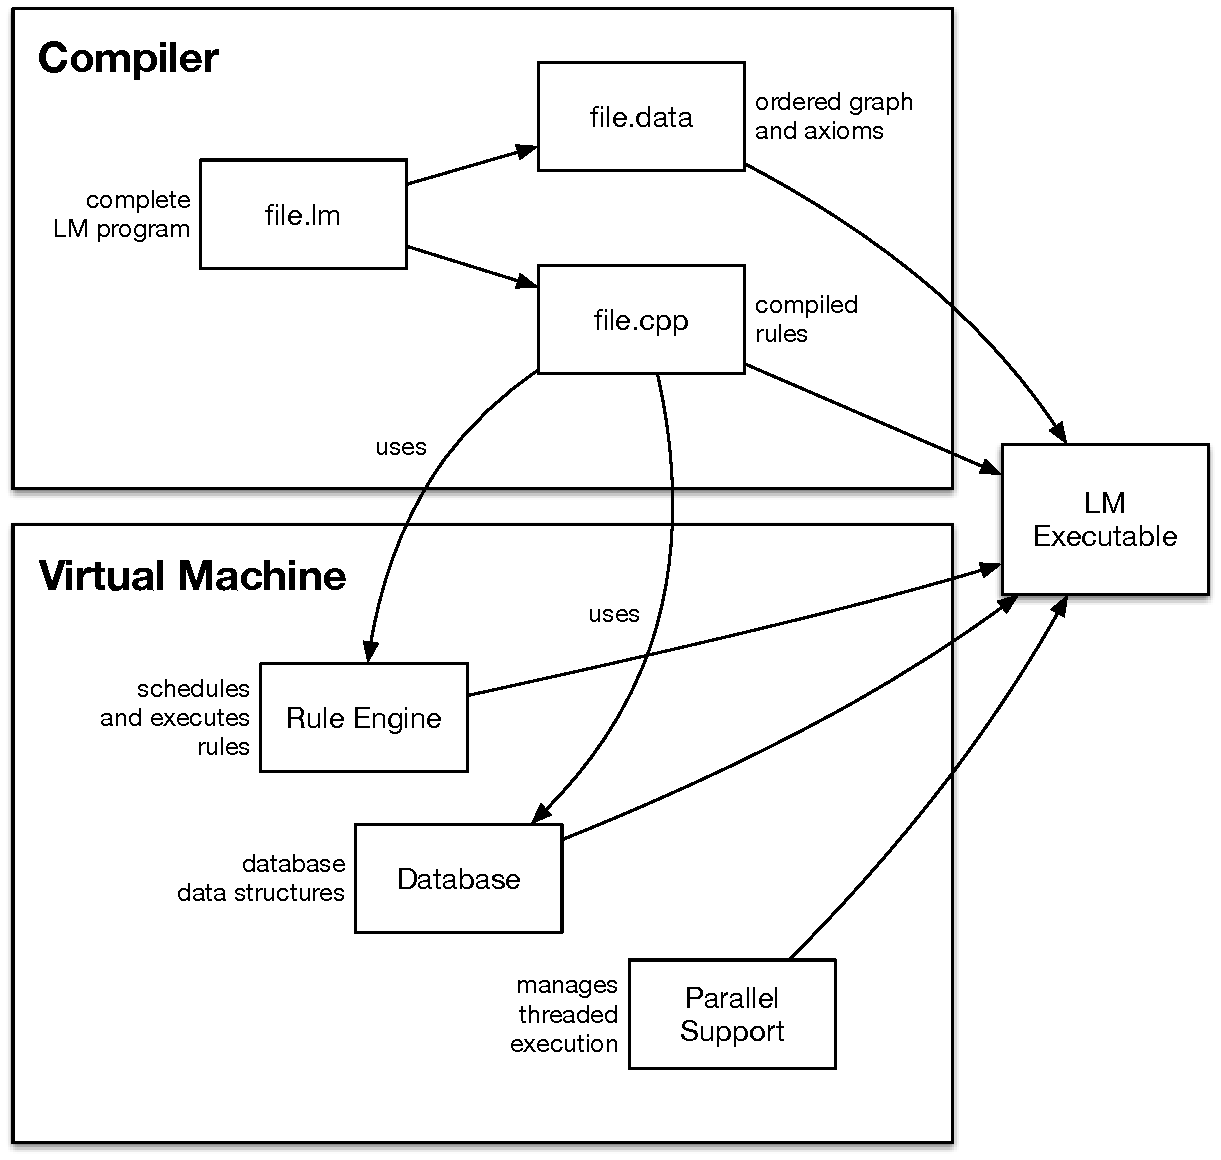
\includegraphics[width=.75\linewidth]{figures/implementation/overview.pdf}

  \mycap{Compilation of a LM program into an executable. The compiler
     transforms a LM program into a C++ file, \code{file.cpp}, with compiled
     rules, and into a data file with the graph structure and initial facts,
     \code{file.data}. The virtual machine which includes code for managing
  multithreaded execution and the database of facts is then linked with both
  files to create a standalone executable that can be run in parallel.}

  \label{fig:implementation:overview}
\end{figure}

The virtual machine contains supporting data structures for managing the
database of facts and to schedule the execution of rules. The parallel engine
described in Chapter~\ref{chapter:implementation} is also a major part of the
virtual machine and is responsible for managing multithreaded execution by
launching threads, managing communication and scheduling concurrent execution.

The compiler transforms LM files into C++ code that uses the virtual machine
facilities to implement the program logic. The compiled code implements the
inference rules of the program and uses the API of the virtual machine to derive
and retract facts and to schedule the execution of rules in the file named
\code{file.cpp}. Since LM does not have traditional input/output facilities, the
compiler also creates a separate file, named \code{file.data}, that contains the
program's initial facts and graph structure and is loaded by the runtime when
the program is executed.

To complete the compilation process, we use a C++ compiler to compile the
virtual machine files and \code{file.cpp} into object files that are then linked
along with \code{file.data}. At the end, we have a standalone executable that
allows the user to input the number of threads to use, program arguments,
facilities to measure run time and also database printing facilities.

Alternatively, the programmer may also decide to compile a more general version
of the virtual machine that is able to run byte-code files generated by the
compiler. This allows faster development since the programmer only needs to
recompile the LM program and not the whole runtime stack. However, LM programs
will run slower since the byte-code must be interpreted by the virtual machine.
This imposes a significant penalty on programs with many mathematical
operations, especially floating point computations.
